%%%%%%%%%%%%%%%%%%%%%%%%%%%%%%%%%%%%%%%%%%%%%%%%%%%%%%%%%%%%%%%%%%%%
% Grundlagen
%%%%%%%%%%%%%%%%%%%%%%%%%%%%%%%%%%%%%%%%%%%%%%%%%%%%%%%%%%%%%%%%%%%%

\chapter{Experiments}
  \label{Exp}
  
This chapter describes the experiments\cite{bekos2019} that were done with this tool in an attempt to validate a proof sketch proposed by Prof. Dr. Mihalis Yannakakis \cite{yannakakis1986four} in 1986.\\
\section{Idea}
As mentioned in \autoref{PR}, Prof. Yannakakis proved in 1986 that all planar graphs can be embedded in at most four stacks \cite{yannakakis1986four,yannakakis1989embedding}. Yet to this day all examined planar graphs were embeddable in three stacks, thus the question remains whether there exists a graph that genuinely requires four stacks.\\
Prof. Yannakakis himself sketched a proof (see \cite{yannakakis1986four}) that utilizes three different graphs who in combination would enable a formal proof for the existence of such a graph. This sketch appeared in an extended abstract of a paper but neither the official version of the paper nor any of his future submissions finalized the proof.
Nevertheless was it subject of intense research and still provides motivation for projects such as the framework this thesis describes.\\
The description of the three graphs are as follows.
\subsection{Step 1}
\label{S1}
The first graph is described by Prof. Yannakakis as a path $p = x_0,x_1,...,x_n$, where $n$ should be sufficiently big (e.g. $n = 1000$). Then add two vertices $A$ and $B$, and connect them to each node $x_i$ of the path (see \autoref{YannakakisGraphs}).\\
This, with a large enough $n$ should lead to a 3-stack linear layout where several consecutive pairs of vertices from path $p$, say  $\langle y_1,y_2 \rangle ... \langle y_{2k-1}, y_{2k}\rangle$ lie in the interval from $A$ to $B$ on the spine.\\
This property is important in order to resume to the second step.
\subsection{Step 2}
\label{S2}
The second graph is a modification of the first, where each of its triangular faces is stellated, that is to say one vertex is added in the center and  connected to each $x_{2k-2}, x_{2k}$ and $A$ (respectively $B$) (see \autoref{S1}).\\
Regarding the subgraph that containts vertices $A, B$ and $y_1,...,y_{2k}$ as well as the newly created $a_1,..,a_k$ and $b_1,...,b_k$, which stellate the faces (see \autoref{YannakakisGraphs}): If k is sufficiently large, this yields a linear layout where four vertices $\langle y_{2i_{0}-1}, a_{i_{0}}, b_{i_0}, y_{2i_{0}}\rangle$ appear on the spine of the linear layout in this order in any corresponding 3-stack layout.

\subsection{Step 3}
\label{S3}
The third modification of the previous graph needs an additional (planar) graph $Q$, which is delimited by the path $(s,a,t,b)$. This graph $Q$ is not fully defined in the proof sketch but should be constructed in a way that it does not admit in a 3-stack layout in which
\begin{itemize}
\item[a)]the partial order of its four vertices is either $(s,a,b,t)$ or $(s,b,a,t)$ or any of the corresponding cyclic rotations and
\item[b)] the edges incident to $s$ and $t$ which connect to vertices that lie in the interval from $s$ to $t$ on the spine of the linear layout, cannot be assigned to the third stack. 
\end{itemize}
Three copies of this graph $Q$ are attached to each edge $(u,v)$ of the original graph such that the vertices $s$ and $t$ of graph $Q$ are replaced by vertices $u,v$.\\[12pt]
Assuming that the base graph is properly constructed through steps one and two, what remains is to find a graph $Q$ with the above mentioned properties.\\
\begin{figure}[h!]
\begin{center}
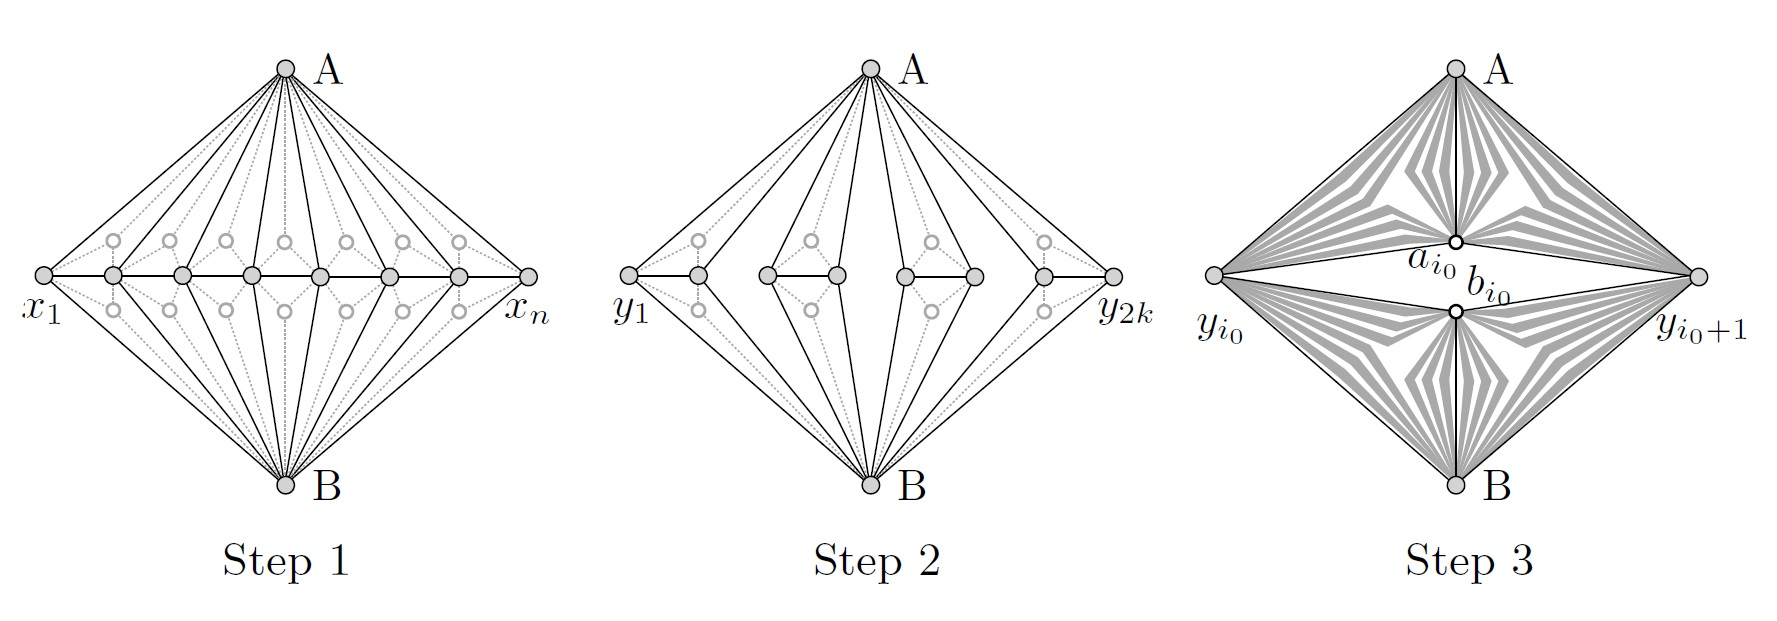
\includegraphics[width=1\textwidth]{figures/yannakakis.jpg}
\caption{Schematic drawings of the constructed graph through all three steps\\ source: \cite{bekos2019}}
\label{YannakakisGraphs}
\end{center}
\end{figure}\\
\section{Our findings}
The first task was to check, whether with a large enough $n$  we could gain a linear layout as described in \autoref{S1}. We constructed the graph with $n = 100$ and imposed constraints according to Prof. Yannakakis idea: vertex $A$ should be a predecessor of every vertex $x_{2i-1}$ and successor of every vertex $x_{2i}$, while vertex $B$ should be a successor of every $x_{2i-1}$ and predecessor of $x_{2i}$. This was done using the \textit{predecessor} constraint described in \autoref{linRestr}.\\
\begin{figure}[h!]
\begin{center}
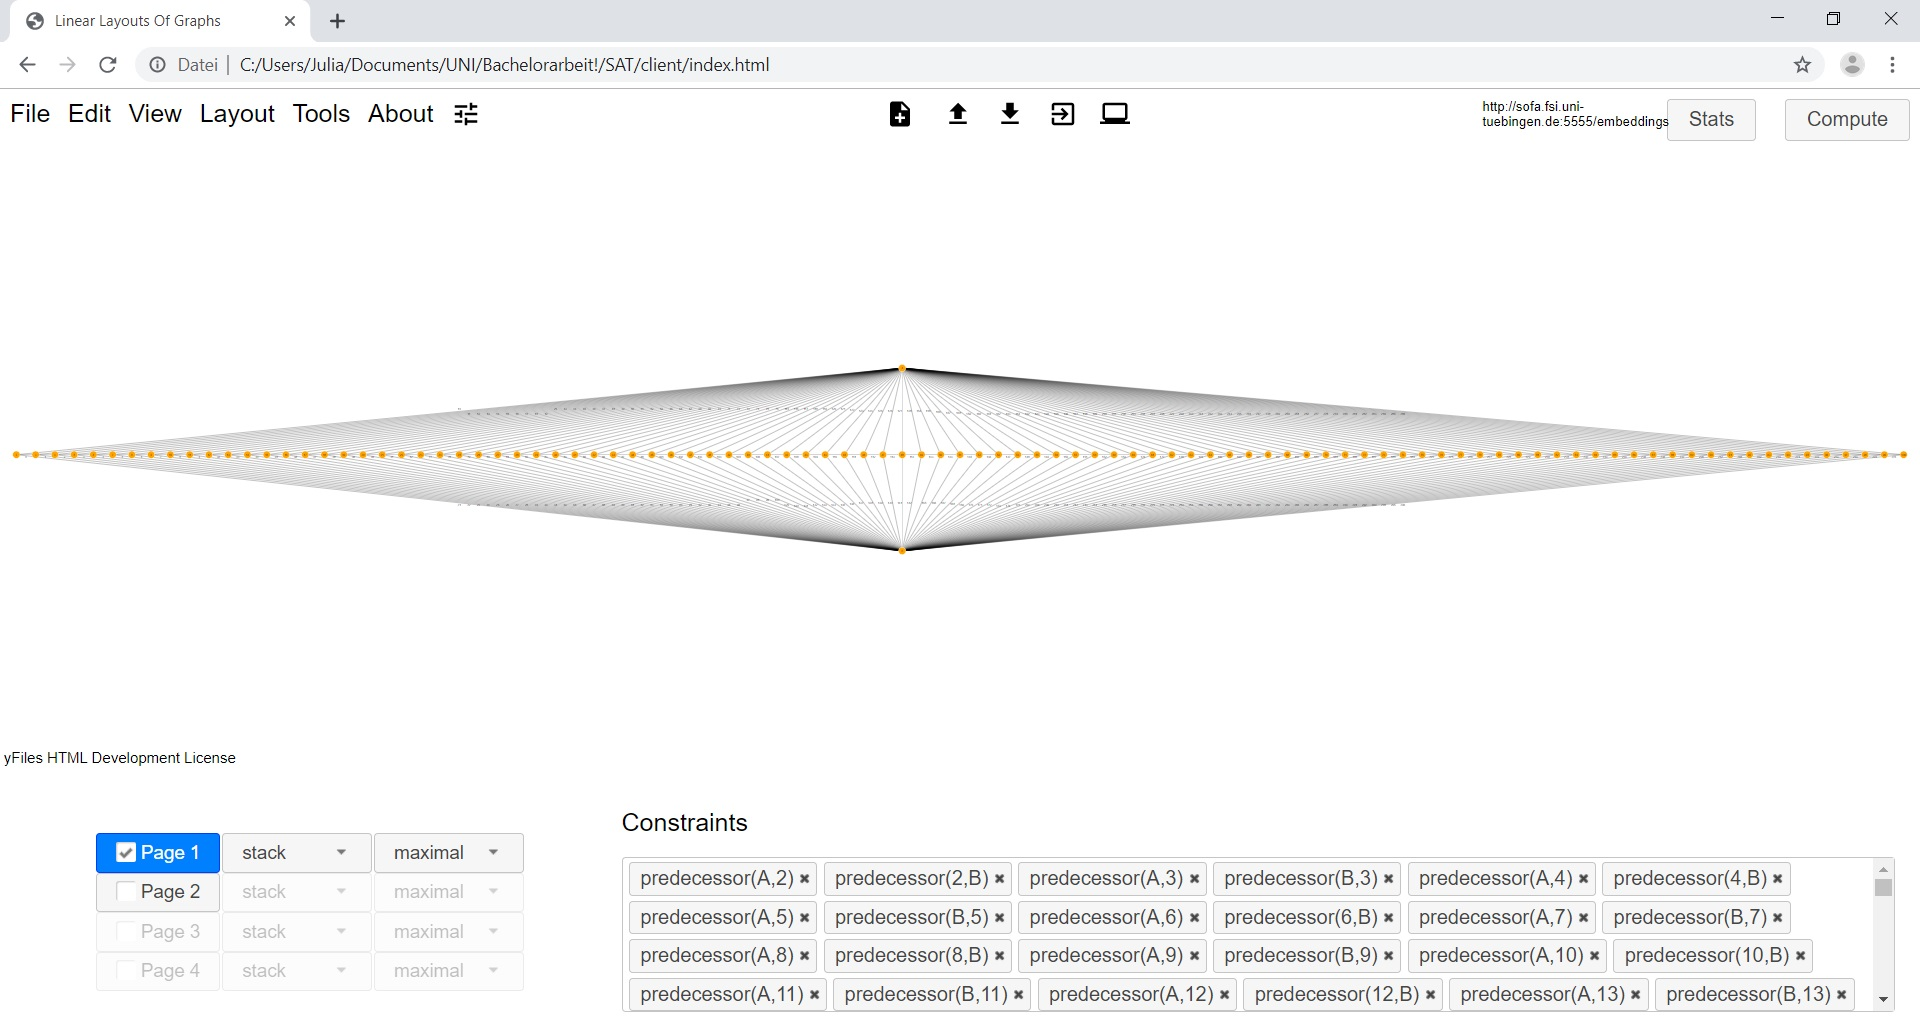
\includegraphics[width=1\textwidth]{figures/skeletonGraph101-296.jpg}
\caption{Our interpretation of the first graph, with 101 vertices and 296 edges as described in \autoref{S1}\label{s1graph}}
\vspace*{24pt}
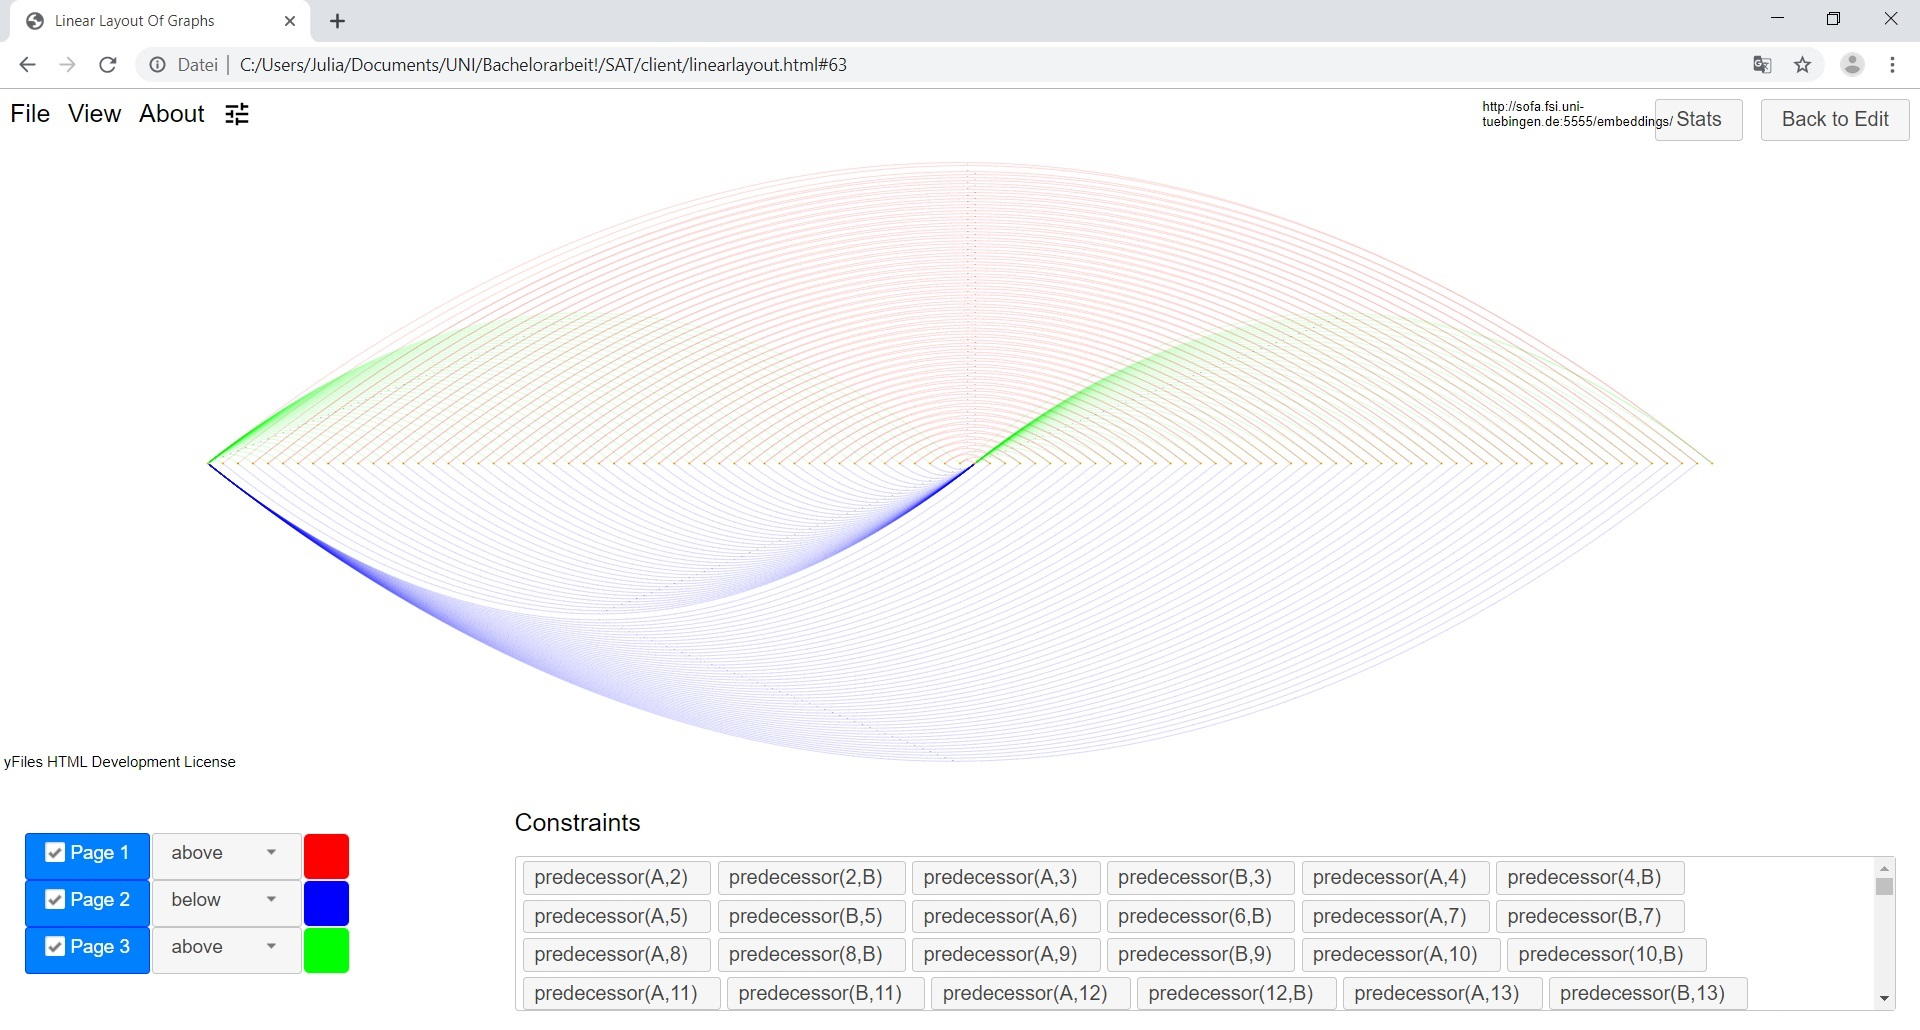
\includegraphics[width=1\textwidth]{figures/skeletonGraph101-296-Solution.jpg}
\caption{The corresponding linear layout to graph in \autoref{s1graph}\label{s1sol}}
\end{center}
\end{figure}
\noindent This 3-stack linear layout turned out to exist, and the edges formed a pattern which could be easily scaled up to any $n$.\\[12pt]
The graph we created according to \autoref{S2} had again $n = 100$ path vertices. The linear layout was constrained in a way that vertex $A$ should be predecessor and $B$ should be successor of all vertices of the graph, for which again the \textit{predecessor} constraint was used. Furthermore for every stellated face the partial orders $\langle y_{2i-1}, a_i, b_i, y_{2i}\rangle$ and $\langle y_{2i-1}, b_i, a_i, y_{2i}\rangle$ were not allowed in the linear layout. This was achieved by using the \textit{restrict partial order} constraint described in \autoref{linRestr}.\\
Again, this yielded a linear layout that admitted a 3-stack layout and was symmetric in a way that increasing $n$ was not necessary.\\
\begin{figure}[h!]
\begin{center}
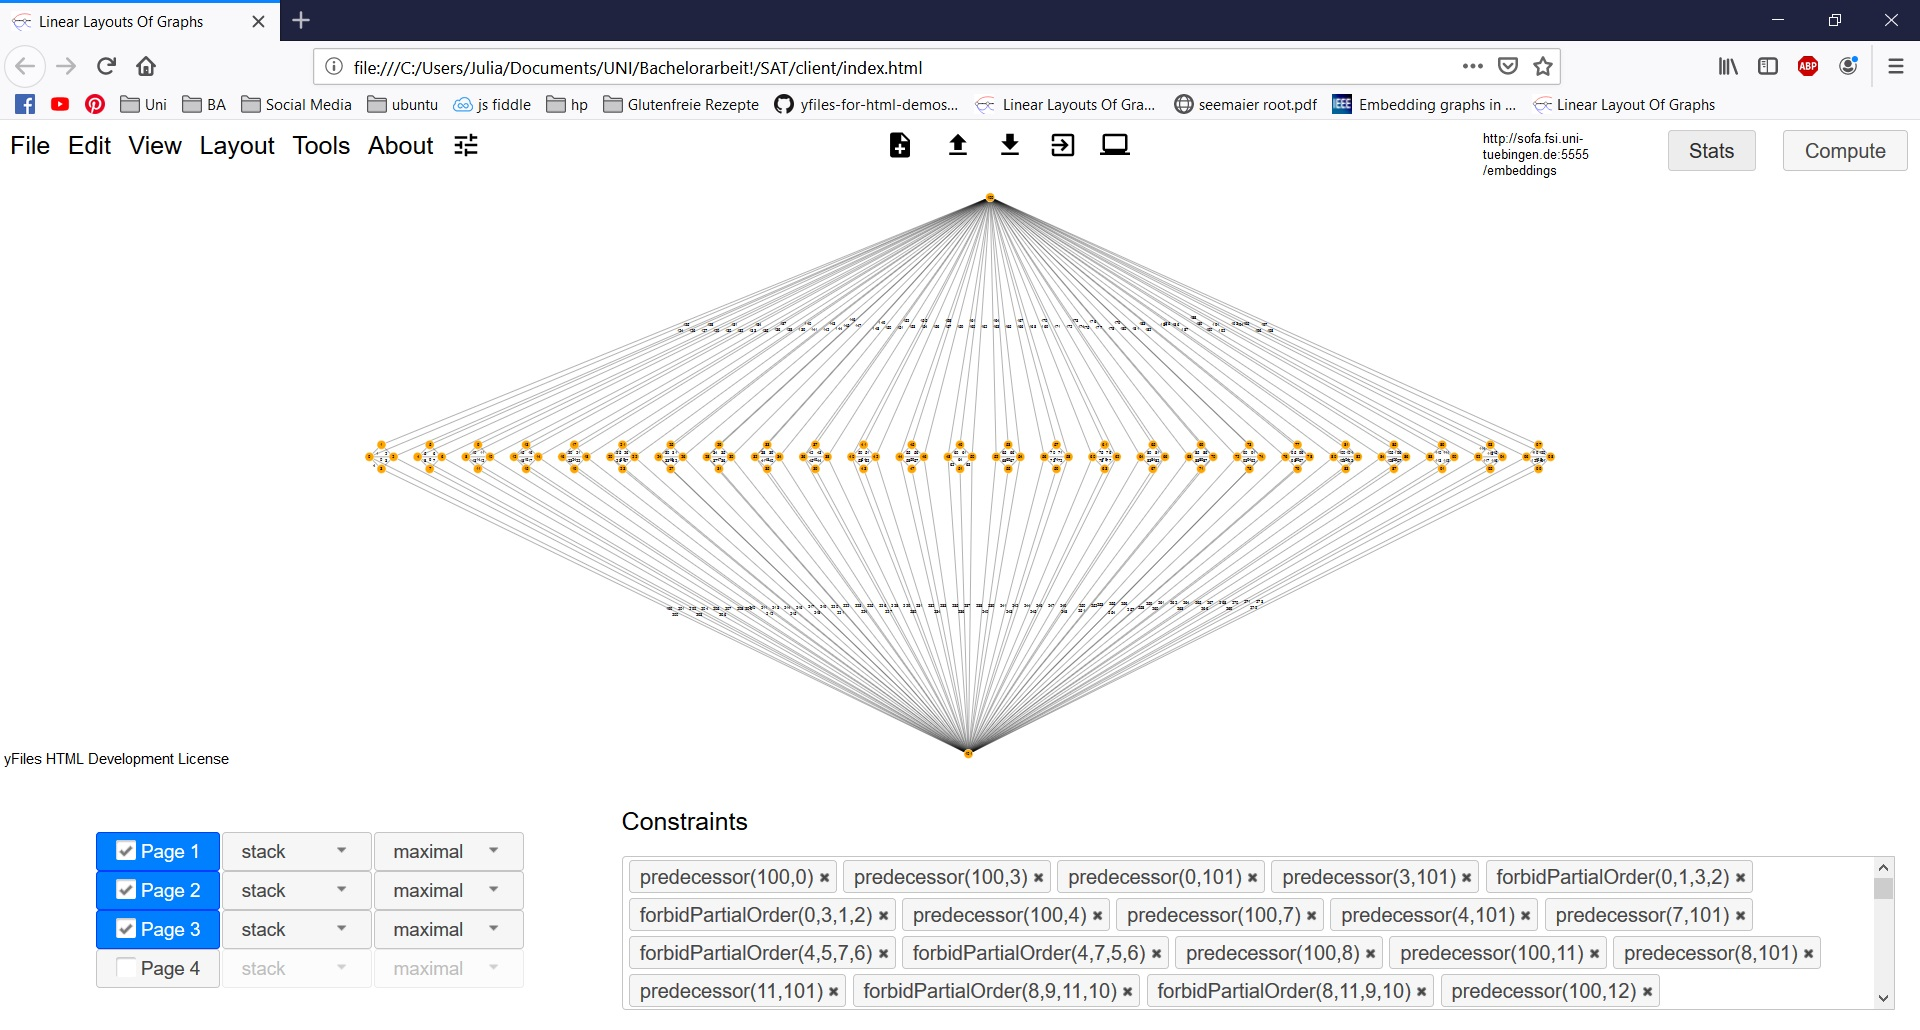
\includegraphics[width=1\textwidth]{figures/stellated-102-274.jpg}
\caption{Our interpretation of the second graph, with 102 vertices and 274 edges as described in \autoref{S2} \label{s2graph}}
\vspace*{24pt}
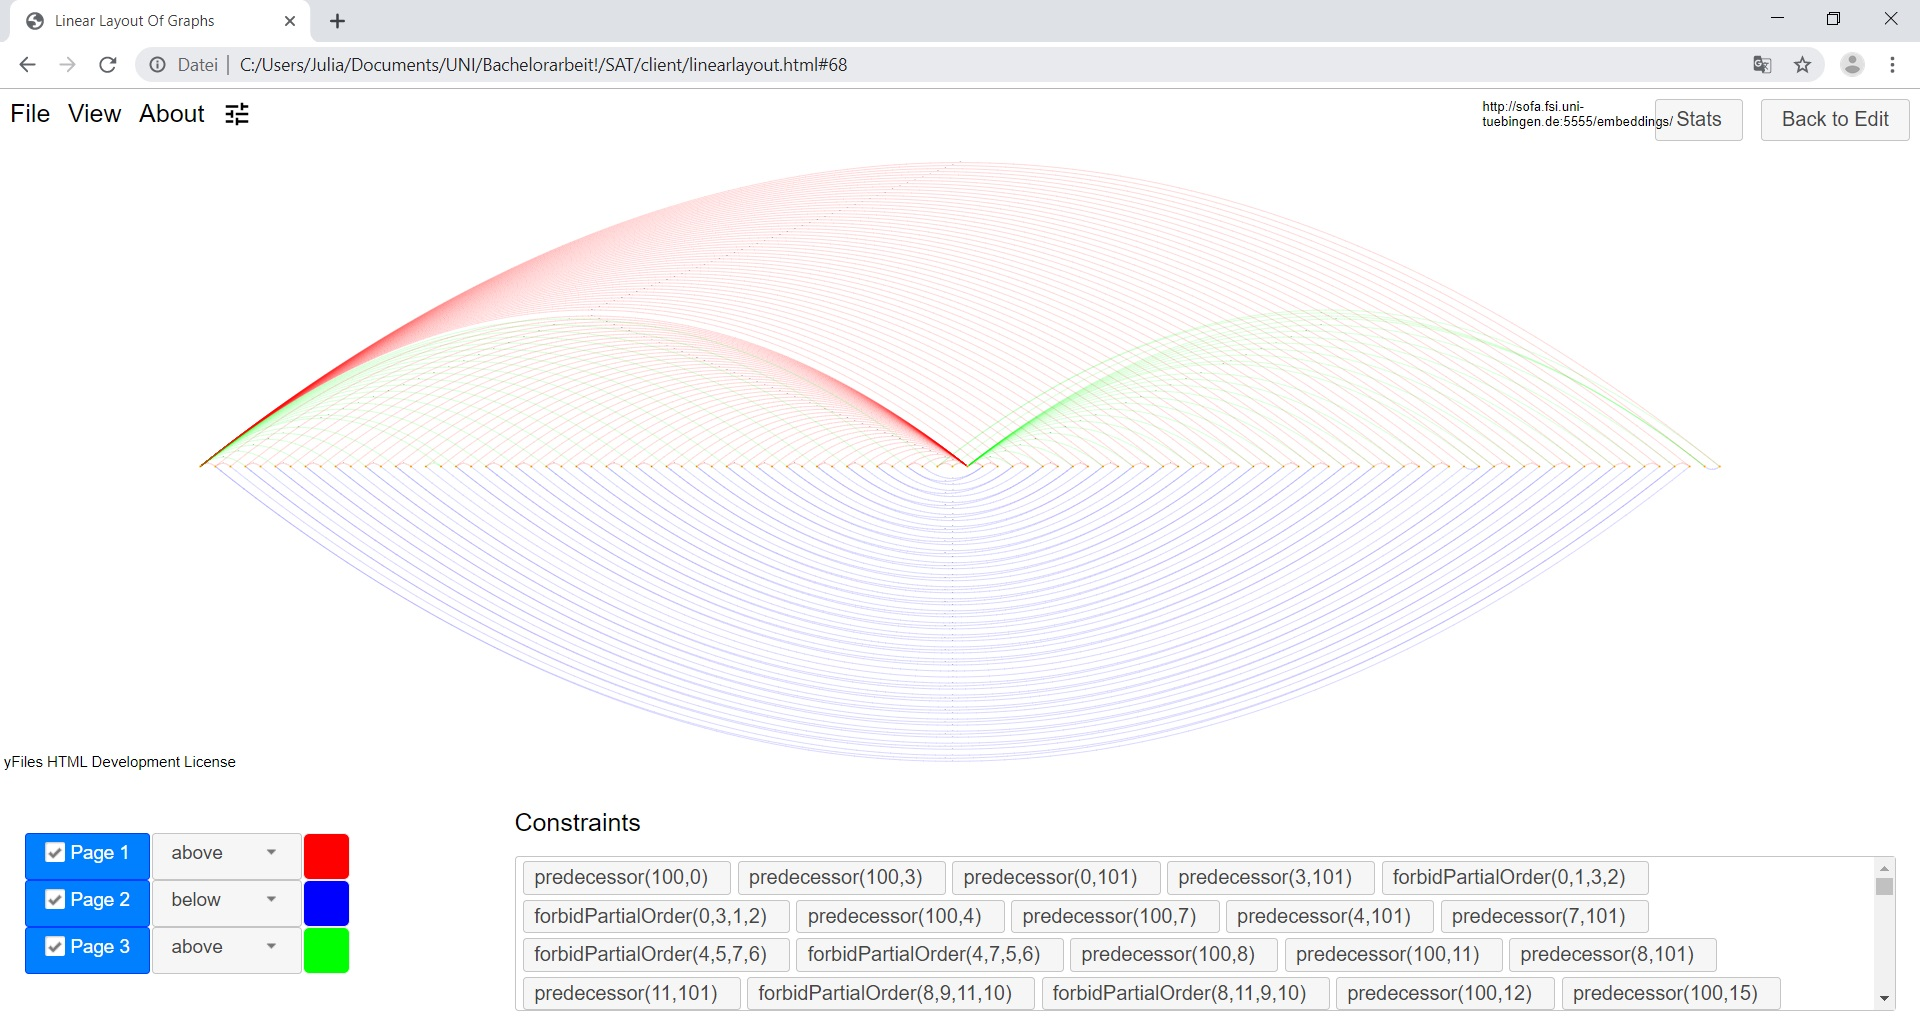
\includegraphics[width=1\textwidth]{figures/stellated-102-274-Solution.jpg}
\caption{The corresponding linear layout to graph in \autoref{s2graph} \label{s2Sol}}
\end{center}
\end{figure}\\
The third part of the proof sketch was not tested using the online framework described in this thesis but by creation of randomly created graphs with constraints following the instructions in \autoref{S3}. The constraint that was necessary to restrict the edges incident from $s$ and $t$ that connect to a vertex in the interval from $s$ to $t$ was nevertheless included in the online framework, (see \autoref{edgeRestr}, \textit{Assign edges incident to certain vertices}). Furthermore the \textit{restrict partial order} constraint was used to exclude the linear orders mentioned in \autoref{S3}. Approximately 4000 random planar graphs with this constraint set  were tested, but all were embeddable in a 3-stack layout. 